% !TEX root = machine_learning.tex
\chapter{Prediction: Basic Concepts}
\label{chap:general}

\section{General Setting}
The goal of prediction is to learn, based on training data, an input-output relationship between two random variables $X$ and $Y$, in the sense of finding, for a specified criterion, the best function of the input $X$ that predicts  the output $Y$. (In statistics, $Y$ is often called the dependent variable, and $X$ the independent variable.) We will, as always, assume that all the variables mentioned in this chapter are defined on a fixed probability space $(\Om, \myP)$. We assume that $X: \Om\to \CR_X$, where $\CR_X$ is the input space, and $Y: \Om \to \CR_Y$, where $\CR_Y$ is the output space. The input-output relationship is therefore captured by an unknown function $f:\CR_X\to\CR_Y$, the predictor.

The following two subclasses of prediction problems are important enough to have learned their own names and specific literature.
\begin{enumerate}[label=$\bullet$,wide]
\item Quantitative output: $\CR_Y = \mR^q$ (often with $q=1$). One then speaks of a {\em regression problem}.
\item Categorical output: $\CR_Y = \{g_1, \dots, g_q\}$ is a finite set. One then speaks of a {\em classification problem}.
\end{enumerate}
In most cases, the input space is Euclidean, i.e., $\CR_X = \mR^d$. Note also that, in classification, instead of a function $f: \CR \to \CR_Y$, one sometimes estimates a function $f:\CR_X \to \boldsymbol\Pi(\CR_Y)$, where $\boldsymbol\Pi(\CR_Y)$ is the space of probability distributions on $\CR_Y$. We will return to this in \cref{rem:pred.prob}.



The quality of a prediction is assessed through the definition of a {\em risk function}.
Such a function, denoted $r$, is defined on $\CR_Y \times \CR_Y$, takes values in $[0, +\infty)$ and should be understood as
\begin{equation}
\label{eq:risk.def}
r(\text{True output}, \text{Predicted output}),
\end{equation}
so that  $r(y,y')$ assigns a cost to the situation in which a true $y$ is predicted by $y'$. 
Note that this definition is asymmetric, and there is no requirement that $r(y,y') = r(y',y)$. It is important to remember our convention that the first variable is the true observation and the second one is a place-holder for a prediction.  
Risk functions are also called {\em loss functions}, or  simply {cost functions} and we will use these terms as synonyms.

The goal in prediction is to minimize the {\em expected risk}, also called the {\em generalization error}:
\[
R(f) = \myE(r(Y, f(X))).
\]

We will prove that an optimal $f$ can be easily described based on the joint distribution of $X$ and $Y$ (which is, unfortunately, never available).
We will need for this to use conditional expectations and conditional probabilities and proceed first to a reminder of their definitions and properties. 

\section{Conditional expectation}
\label{sec:cond.exp}

If $\boldsymbol \xi:\Omega \to \CR_\xi$ and $\boldsymbol\eta:\Omega \to \CR_\eta\subset \mR^d$ are discrete random variables, then
\[
\myP(\boldsymbol\eta=\eta \mid \boldsymbol\xi=\xi) = \myP(\boldsymbol\eta=\eta, \boldsymbol\xi=\xi)/\myP(\boldsymbol\xi=\xi)
\]
if $\myP(\boldsymbol\xi =\xi) >0$ and is undefined otherwise. Then, if $\bfeta$ is real-valued and discrete, one defines the conditional expectation of $\bfeta$ given $\bfxi$, denoted $\myE(\bfeta\mid \bfxi)$, by
\[
\myE(\bfeta\mid \bfxi)(\om) = \sum_{\eta\in \CR_\eta} \eta \myP(\bfeta =\eta \mid \bfxi=\bfxi(\om))
\]
for all $\om$ such that $\myP(\bfxi=\bfxi(\om))>0$. Note that $\myE(\bfeta\mid \bfxi)$ is a random variable, defined over $\Om$. It however only depends on the values of $\bfxi$, in the sense that $\myE(\bfeta\mid \bfxi)(\om) = \myE(\bfeta\mid \bfxi)(\om')$ if $\bfxi(\om) = \bfxi(\om')$. We will use the notation 
\[
\myE(\bfeta\mid \bfxi=\xi) = \sum_{\eta\in \CR_\eta} \eta \myP(\bfeta=\eta \mid \bfxi=\xi), 
\]
which is now a function defined on $\CR_\xi$.
One has $\myE(\bfeta\mid \bfxi)(\om) = \myE(\bfeta \mid \bfxi=\bfxi(\om))$.
 
One can characterize $\myE(\bfeta\mid \bfxi)$ by the properties
\begin{equation}
\label{eq:cond.exp}
\begin{cases}
\myE(\bfeta\mid \bfxi) \text{ is a function of $\bfxi$}\\
\forall f: \CR_\eta \to \mR, \myE(\myE(\bfeta\mid \bfxi) f(\bfxi)) = \myE(\bfeta f(\bfxi)).
\end{cases}
\end{equation}
The proof that our definition of $\myE(\bfeta\mid \bfxi)$ for discrete random variables is the only one satisfying these properties is left to the reader. The interest of reformulating the definition of the conditional expectation via \cref{eq:cond.exp} is that this provides a definition that works for general random variables (with the additional assumption that $f$ is measurable), not only for discrete ones. We assume below that $(\CR_\xi, \boldsymbol{\CS}_\xi)$ and $(\CR_\eta, \boldsymbol{\CS}_\eta)$ are measurable spaces.

\begin{definition}
\label{def:cond.exp}
Assume that $\CR_\eta = \mR^d$.
Let $\bfxi: \Om\to \CR_\xi$ and $\bfeta:\Om \to \CR_\eta$ be two random variables with  $\myE(|\bfeta|) <\infty$. The conditional expectation of $\bfeta$ given $\bfxi$ is a random variable $\bfzeta: \Om \to \CR_\eta$ such that
\begin{enumerate}[label = (\roman*),wide=0pt]
\item There exists a function $h: \CR_\xi \to \mR$ such that $\zeta = h 
\circ \bfxi$ almost surely.
\item For any measurable function $g: \CR_\xi \to [0, +\infty)$, one has
\[
\myE(\bfeta g\circ \bfxi) = \myE(\bfzeta g\circ \bfxi).
\]
\end{enumerate}
The variable $\bfzeta$ is then denoted $\myE(\bfeta|\bfxi)$ and the function $h$ in (i) is denoted $\myE(\bfeta|\bfxi = \cdot)$.
\end{definition}

Importantly, functions $\bfzeta$ satisfying conditions (i) and (ii) always exists and are almost surely unique,  in the sense that if another function $\bfzeta'$ satisfies these conditions, then $\bfzeta = \bfzeta'$ with probability one. One obtains an equivalent definition if one restricts functions $g$ in (ii) to indicators of measurable sets, yielding the condition that, if $A\subset \CR_\xi$ is measurable,
\[
\myE(\bfeta \bfone_{\bfxi\in B} ) = \myE(\bfzeta \bfone_{\bfxi\in B}).
\]


Taking $g(\xi) = 1$ for all $\xi\in \CR_\xi$ in condition (ii), one gets the well-known identity
\[
\myE(\myE(\bfeta|\bfxi)) = \myE(\bfeta).
\]
Moreover, for any function $g$ defined on $\CR_\xi$ we have $\myE(\bfeta g\circ \bfxi|\bfxi) = (g\circ \bfxi)  \myE(\bfeta|\bfxi)$, which can be checked by proving that the right-hand side satisfies the conditions (i) and (ii).



Conditional expectations share many of the properties of simple expectations. For example, if $\bfeta \leq \bfeta'$, both taking scalar values, then $\myE(\bfeta\mid\bfxi) \leq \myE(\bfeta'\mid \bfxi)$ almost surely. Jensen's inequality also holds: if $\gamma: \mR^d\to \mR$ is convex and $\gamma\circ \bfeta$ is integrable, then
\[
\gamma\circ \myE(\bfeta\mid \bfxi) \leq \myE(\gamma \circ \bfeta \mid \xi).
\]
We will discuss convex functions in \cref{chap:optim}, but two important examples for this section are $\gamma(\eta) = |\eta|$ and $\gamma(\eta) = |\eta|^2$. The first one implies that $|\myE(\bfeta\mid \bfxi)| \leq \myE(|\bfeta|\mid bfxi)$ and, taking expectations on both sides:  $\myE(|\myE(\bfeta\mid \bfxi)|) \leq \myE(|\bfeta|)$, the upper bound being finite by assumption. For the square norm, we find that, if $\eta$ is square integrable, then so is $\myE(\bfeta\mid \bfxi)$ and 
\[
\myE(|\myE(\bfeta\mid \bfxi)|^2) \leq \myE(|\bfeta|^2).
\]

If $\bfeta$ is square integrable, then this inequality shows that $\myE(\bfeta\mid \bfxi)$ minimizes $\myE[|\bfeta - \bfzeta|^2]$ among all square integrable functions $\zeta:\Om\to \CR_\eta$ that satisfy (i). In other terms, the conditional expectation is the optimal least-square approximation of $\bfeta$ by a function of $\bfxi$. To see this, just write
\begin{align*}
\myE[|\bfeta - \bfzeta|^2\mid \bfxi] &= \myE[|\bfeta|^2\mid \bfxi]  - 2\myE[\bfeta^T\bfzeta\mid\bfxi]
+ |\bfzeta|^2\\
&= \myE[|\bfeta|^2\mid\bfxi]  - 2\myE(\bfeta\mid\bfxi)^T\bfzeta
+|\bfzeta|^2\\
&= \myE[|\bfeta|^2\mid\bfxi] - |\myE(\bfeta\mid\bfxi)|^2 +|\myE(\bfeta\mid\bfxi) -\bfzeta|^2\\
&= \myE[|\bfeta - \myE(\bfeta\mid\bfxi)|^2\mid\bfxi] +|\myE(\bfeta\mid\bfxi) -\bfzeta|^2\\
&\geq \myE[|\bfeta - \myE(\bfeta\mid\bfxi)|^2\mid\bfxi]
\end{align*}
and taking expectations on both sides yields the desired result.


If $A$ is a measurable subset of $\CR_\eta$, the conditional expectation $\myE(\bfone_A\mid \bfxi)$ (resp. $\myE(\bfone_A\mid \bfxi = \xi)$) is denoted  $\myP(\bfeta \in A\mid \bfxi)$ (resp. $\myP(\bfeta\in A\mid \bfxi = \xi)$), or $P_\bfeta(A\mid \bfxi)$ (resp. $P_\bfeta(A\mid \bfxi = \xi)$).
While these functions are defined separately up to modifications on sets of probability zero. Under general assumptions on the set $\CR_\eta$ and its $\sigma$-algebra (always satisfied in our discussions), these conditional probabilities can be defined together so that, for all $\omega \in \Omega$  $A\mapsto P_\bfeta(A \mid \bfxi)(\omega)$ is a probability distribution  on $\CR_\eta$ such that
\[
\myE(\bfeta\mid \bfxi) = \int_{\CR_\eta} \eta \myP(d\eta\mid \bfxi).
\] 

Assume that the the sets $\CR_\xi$ and $\CR_\eta$ are equipped with measures, say $\mu_\xi$ and $\mu_\eta$ such that the joint distribution of $(\xi,  \eta)$ is absolutely continuous with respect to $\mu\xi\otimes \mu_\eta$, so that there exists a function $\phi:\CR_\xi\times \CR_\eta\to \mR$ (the p.d.f. of $(\xi, \eta)$ with respect to $\mu\xi\otimes \mu_\eta$) such that 
\[
\myP(\bfxi\in A, \bfeta\in B) = \int_{A\times B} \phi(\xi, \eta) \mu_\xi\otimes \mu_\eta(dx, d\eta).
\]
Then $P_\bfeta(\cdot\mid \xi)$ is absolutely continuous with respect to $\mu_\eta$, with density given by the conditional p.d.f. of $\bfeta$ given $\bfxi$, namely,
\begin{equation}
\label{eq:cond.pdf}
\phi(\cdot\mid \bfxi): (\eta, \om) \mapsto \frac{\phi(\eta, \bfxi(\om))}{\int_{\CR_\eta} \phi(\eta',\bfxi(\om))\, \mu_\eta(d\eta')} = \phi(\eta\mid \bfxi= \bfxi(\omega)).
\end{equation}
Note that 
\[
\myP\left\{\omega: \int_{\CR_\eta} \phi(\eta',\bfxi(\om))\, \mu_\eta(d\eta') = 0\right \} = 0
\]
so that the conditional density can be defined arbitrarily when the numerator vanishes\footnote{Letting $\phi_\xi(\xi) = \int_{\CR_\eta}\phi(\eta',\xi)\, \mu_\eta(d\eta')$, which is the marginal p.d.f. of $\bfxi$ with respect to $\mu_\xi$, we have
\[
\myP(\phi_\xi(\bfxi)= 0) = \int_{\CR_\xi} \bfone_{\phi_\xi(\xi)= 0} \phi_\xi(\xi) \mu_\xi(d\xi) = 0.
\] 
}.

The most common example is when $\CR_\xi$ and $\CR_\eta$ are Euclidean spaces and $\mu_\xi$, $\mu_\eta$ are Lebesgue's measures, in which case \cref{eq:cond.pdf} is the usual definition of conditional p.d.f.'s. Note also that, for discrete random variables, \cref{eq:cond.pdf} coincides with the definition of conditional probabilities $\myP(\bfeta = \eta \mid \bfxi = \bfxi(\omega))$ when $\mu_x$ and $\mu_\eta$ are counting measures. As a last example, if $\CR_\xi = \mR^d$, $\mu_\xi$ is Lebesgue's measure and $\bfeta$ is discrete, then
\[
\phi(\eta \mid \bfxi = \bfxi(\omega) ) = \frac{\phi(\eta, \bfxi(\om))}{\sum_{\eta' \in \CR_\eta} \phi(\eta',\bfxi(\om))}.
\]

%
%If $A\subset \CR_\xi$ and $\myP(\bfxi \in A) >0$, the conditional probability 
%\[
%\myP(\bfeta\in B \mid \bfxi \in A) = \frac{\myP(\bfeta \in B \text{ and }\bfxi \in A)}{\myP(\bfxi\in A)}
%\]
% is well defined, and one can write
%\[
%\myE(\bfeta \mid\bfxi\in A) = \frac{1}{\myP(\bfxi\in A)} \myE(\bfeta\bfone_{\eta\in A})
%\]
%so that
%%\footnote{We will use the  notation $\bfone_{\text{event}}$ as the random variable equal to 1 when the event is true and to 0 otherwise.}
%$\myP(\bfeta\in B \mid\bfxi \in A) = \myE(\bfone_{\bfeta \in B}\mid \bfxi \in B)$. 
%
%
%If $\xi\in \CR_\xi$, the conditional probability $\myP(\bfeta\in B \mid \bfxi = \xi)$ is not so easy to define, because, very often, $\myP(\bfxi= \xi) = 0$ for all $\xi$. It is a somewhat technical result in probability theory that, under mild assumptions on the considered spaces, such a $\xi$-indexed family of probability distributions can be defined with the property that, for any function $f:\CR_\eta \to\mR$,
%$\myE(f(\bfeta)\mid \bfxi)(\om)$ coincides with the integral of $f(\bfeta)$ with respect to the measure $B \mapsto \myP(\bfeta\in B \mid \bfxi = \bfxi(\om))$. 
%\medskip
%
%In this book, we will almost always be in one, or a mixture of, of the following cases:
%\begin{enumerate}[wide]
%\item $\CX = \mR^d$ and $\CY = \mR^q$ with joint p.d.f. $f$, in which case $B \mapsto \myP(\xi\in B | \eta = y)$ has p.d.f. 
%\[
%f(x|y) = \frac{f(x,y)}{\int_{\mR^d} f(x', y)\, dx'}.
%\]
%\item $\CY$ is finite, in which case the conditional distribution is easy to define.
%\end{enumerate}
%\bigskip

\section{Bayes predictor}
\label{sec:bayes.pred}
Recall that $r: (y,y')\mapsto r(y,y')$ denotes the risk function and that we want to minimize $R(f) = \myE(r(Y, f(X))$ over all possible predictors $f$. 
\begin{definition}
\label{def:bayes.pred}
A Bayes predictor is a measurable function $f: \CR_X \to \CR_Y$ such that, for all $x\in \CR_X$, 
\[
\myE\big(r(Y, f(x))\mid X=x\big) = \min\big\{\myE\big(r(Y, y')\mid X=x\big): y'\in \CR_Y\big\}
\]
\end{definition}
There can be multiple Bayes predictors if the minimum in the proposition is not uniquely attained.
Note that, if $f^{*}$ is a Bayes predictor and $\hf$ any other predictor, we have, by definition 
\[
\myE\big(r(Y, f^{*}(X))\mid X\big) \leq \myE\big(r(Y, \hf(X))\mid X\big).
\]
Passing to expectations, this implies $R(f^{*}) \leq R(\hf)$. We therefore have the following result:
\begin{theorem}
\label{th:bayes.pred}
Any Bayes predictor 
 $f^{*}$ is optimal, in the sense that it minimizes the generalization error $R$.
 \end{theorem}


\begin{enumerate}[label= Example \arabic*., wide=0pt, font=\itshape]
\item {\it Regression with mean-square error.} When $\CR_X = \mR^d$ and $\CR_Y = \mR^{q}$, the most common  risk function is the squared norm $r(y,y') = |y-y'|^{2}$. 
The resulting generalization error is called the MSE (mean square error) and given by $R(f) = \myE(|Y-f(X)|^{2})$.
The Bayes predictor is such that $f^{*}(x)$ minimizes 
\[
t \mapsto \myE(|Y-t|^{2}\mid X=x).
\]
Let $f^{*}(x) = E(Y\mid X=x)$ and write
\begin{align*}
\myE(|Y-t|^{2}\mid X=x) =& \myE(|Y-f^*(x)|^{2}\mid X=x) + 2 \myE((Y-f^*(x))^T(f^*(x)-t)\mid X=x) \\
&+ |f^*(x) - t|^2\\
=& \myE(|Y-f^*(x)|^{2}\mid X=x) + 2 \myE((Y-f^*(x))^T\mid X=x)(f^*(x)-t) \\
&+ |f^*(x) - t|^2\\
=& \myE(|Y-f^*(x)|^{2}\mid X=x) + |f^*(x) - t|^2.
\end{align*}
This proves that $\myE(Y\mid X=x)$ is the unique Bayes classifier (up to a modification on a set of probability 0).
\label{item:Bayes.MSE}
\item {\it Classification with zero-one loss.}
Let $\CR_X = \mR^d$ and $\CR_Y$ be a finite set. The zero-one loss function is defined by  $r(y,y') = 1$ if $y\neq y'$ and 0 otherwise.
From this, it results that the generalization error is the probability of misclassification $R(f) = P(Y\neq f(X))$ (also called the misclassification error).

The Bayes predictor is such that $f^{*}(x)$ minimizes 
\[
g \mapsto \myP(Y\neq g\mid X=x) = 1 - \myP(Y = g\mid X=x).
\]
It is therefore given by the so-called {\it posterior  mode}:
\[
f^{*}(x) = \mathrm{argmax}_{g} \myP(Y = g\mid X=x).
\]
\end{enumerate}

\begin{remark}
\label{rem:pred.prob}
As mentioned at the beginning of the chapter, one sometimes replaces a pointwise prediction of the output by a probabilistic one, so that $f(x)$ is a probability distribution on $\CR_Y$. If $A$ is a (measurable) subset of $\CR_Y$, we will write $f(x, A)$ rather than $f(x)(A)$. 

In such a case, the loss function, $r$, is defined on $\CR_Y \times \boldsymbol\Pi(\CR_Y)$, and the expected risk is still defined by
$\myE(r(Y, f(X)))$.

It is quite natural to require that $\pi \mapsto r(y, \pi)$ is minimized. For classification problems, where $\CR_Y$ is finite, one can choose
\begin{equation}
\label{eq:risk.mle}
r(y, \pi) = - \log \pi(y)
\end{equation}
The Bayes estimator is then a minimizer of $\pi \mapsto -\myE(\log\pi(Y)\mid X=x)$. The solution is (unsurprisingly) $f(x,y) = \myP(Y=y \mid X=x) $ since we always have
\[
-\myE(\log\pi(Y)\mid X=x) = -\sum_{y\in\CR_Y} \log\pi(y) f(x,y) \geq  -\sum_{y\in\CR_Y} \log f(x,y) f(x,y).
\]
The difference between these terms is indeed
\[
\sum_{y\in\CR_Y} \log \frac{f(x,y)}{\pi(y)} f(x,y) = \KL(f(x, \cdot), \pi) \geq 0.
\]

For regression problems, with $\CR_Y = \mR^q$, one can choose
\[
r(y, \pi) = \int_{\mR^q} |z - y|^2 \pi(dz)
\]
which is indeed minimum when $\pi$ is concentrated on $y$. Here, the Bayes estimator minimizes (with respect to $\pi$)
\[
\int_{\mR^q} \int_{\mR^q} |z - y|^2 \pi(dz) P_Y(x, dy) = \int_{\mR^q} \left(\int_{\mR^q} |z - y|^2 P_Y(x, dy)\right) \pi(dz) 
\]
where $P_Y(x, \cdot)$ is the conditional distribution of $Y$ given $X=x$. For any $z$, one has
\[
\int_{\mR^q} |y - z|^2 f(x, dy) \geq \int_{\mR^q} |y - \myE(Y\mid X=x)|^2 f(x, dy)
\]
which shows that the Bayes estimator is, in this case, the Dirac measure concentrated at $\myE(Y\mid X=x)$.

\end{remark}

\section{Examples: model-based approach}
Bayes predictors are never  available in practice, because the
true distribution of $(X,Y)$, or that of $Y$ given $X$, are unknown. These distributions can only be inferred from observations, i.e., from a training set: $T = (x_1, y_1,
\ldots, x_N, y_N)$. 

This is the approach followed by {\em model-based}, or {\em generative} methods, namely using training data to approximate the joint distribution of $X$ and $Y$ with a statistical model estimated from data before using the Bayes estimator derived from this model for prediction. We now illustrate this approach with a few examples.

\subsection{Gaussian models and naive Bayes}
Consider a regression problem with $\CR_Y = \mR$, and model the joint distribution of $(X, Y)$ as a $(d+1)$-dimensional Gaussian distribution with mean $\mu$ and covariance matrix $\Sigma$, which must be estimated from data.
Write $\mu =\begin{pmatrix} m \\\mu_{0}\end{pmatrix}$, with $\mu_0\in\mR$, $m\in \mR^{d}$ and $\Sig$ in the form, for some symmetric matrix $S$ and $d$-dimensional vector $u$
%\footnote{We  denote by $\Id_{\mR^{d}}$ the $d$-dimensional identity matrix}
\[
\Sig = \begin{pmatrix} S  & u\\  u^{T} & \sig^{2}_{00} \end{pmatrix}.
\]
Then,  letting $\Delta = \sig^{2}_{00} - u^{T }S^{-1}u$,
\[
\Sig^{{-1}} = \frac1 \Delta \begin{pmatrix}\Delta S^{-1} +  S^{-1}uu^{T}S^{-1} & -S^{-1}u \\  - u^{T}S^{-1} & 1 \end{pmatrix}\,.
\]

This shows that the joint p.d.f. of $(X,Y)$ is proportional to
\begin{multline*}
\exp\Big(-\frac1{2\Delta} \big((y-\mu_{0})^{2} - 2 u^{T}S^{-1} (x-m)(y-\mu_{0})
+ \text{(\it terms not depending on $y$)} \big)\Big).
\end{multline*}
In particular
\[
E(Y|X) = \mu_{0} + u^{T} S^{-1}(x-m),
\]
which provides the least-square linear regression predictor. (In this expression, $u$ is the covariance between $X$ and $Y$ and $S$ is the covariance matrix of $X$.)
\bigskip

If one restricts the model to having  a diagonal covariance matrix $S$, then
%\footnote{We will generally use parentheses to denote vector coordinates: $x = (x(1), \ldots, x(d))^{T}$.}
\[
E(Y|X) = \mu_{0} + \sum_{j=1}^{d} \frac{\pe u j }{s_{jj}} (\pe x j  -\pe  m j ).
\]
This predictor is often called the {\em naive Bayes} predictor for regression.

\subsection{Kernel regression}
Let $\CR_X = \mR^{d}$ and $\CR_Y = \mR$.
Let $K_{1}: \mR^{d} \to \mR$ and $K_{2}: \mR \to \mR$ be two kernels, therefore satisfying
\[
\int_{\mR^{d}} K_{1}(x) dx = \int_{\mR} K_{2}(x) dx = 1;\quad \int_{\mR^{d}} xK_{1}(x) dx = \int_{\mR} yK_{2}(y) dy = 0.
\]
Let $K(x,y) = K_{1}(x) K_{2}(y)$ so that
\[
\begin{aligned}
&\int_{\mR^{d+1}} K(x,y) dydx = 1\\
& \int_{\mR^{d+1}} yK(y,x) dydx = 0\\
&\int_{\mR^{d+1}} xK(y,x) dydx = 0.
\end{aligned}
\]

The kernel estimator of the  joint p.d.f., $\phi$, of $(X,Y)$ at
scale $\sig$ is, in this case:
$$
\hat\phi(x,y) = \frac{1}{N} \sum_{k=1}^N \frac{1}{\sig^{d+1}}
K_1\left(\frac{x-x_k}{\sig}\right)K_2\left(\frac{y-y_k}{\sig}\right)\, .
$$
Based on $\hat\phi$, the conditional expectation of $Y$ given $X$ is
$$
\hf(x) = \frac{\frac{1}{N} \sum_{k=1}^N \frac{1}{\sig^{d+1}} \int_{\mR} y
K_1\left(\frac{x-x_k}{\sig}\right)K_2\left(\frac{y-y_k}{\sig}\right)
dy}{\frac{1}{N} \sum_{k=1}^N \frac{1}{\sig^{d+1}} \int_{\mR} 
K_1\left(\frac{x-x_k}{\sig}\right)K_2\left(\frac{y-y_k}{\sig}\right) dy}\, .
$$

Using the fact that
$\sig^{-1}\int_{\mR} y
K_2\left(\frac{y-y_k}{\sig}\right) dy = y_k$, we can simplify this expression to obtain
$$
\hf(x) = \frac{ \sum_{k=1}^N  y_k 
K_1\left(\frac{x-x_k}{\sig}\right)}{ \sum_{k=1}^N 
K_1\left(\frac{x-x_k}{\sig}\right)} \,.
$$
This the kernel-density regression estimator \citep{nadaraya1964estimating,watson1964smooth}.

\subsection{A classification example}
Let $\CR_Y = \{0,1\}$ and assume $\CR_X = \mathbb N =  \{0,1,2,\ldots\}$.
Let $p = \myP(Y=1)$ and assume that conditionally to $Y=g$, $X$ follows a Poisson distribution with mean $\mu_{g}$. Assume that $\mu_{0 }< \mu_1$.

The posterior distribution of $Y$ given $X=x$ is\,\footnote{$\propto$ is the notation for ``proportional to''}
\[
\myP(Y=g\mid X=x) \propto \left\{
\begin{aligned}
(1-p)\mu_{0}^{x}e^{-\mu_0} \text{ if } g=0\\
p\mu_{1}^{x}e^{-\mu_1} \text{ if } g=1
\end{aligned}
\right.
\]

A Bayes classifier is then provided by taking $f(x) = 1$ if
\[
\log p + x\log \mu_1 - \mu_1 \geq \log(1-p) + x\log\mu_0 - \mu_0
\]
that is:
\[
x \log\frac{\mu_1}{\mu_0} \geq \log \frac{1-p}{p} + \mu_1 - \mu_0
\]
Since we are assuming that $\mu_1 > \mu_0$, we find that $f(x) = 1$ if\,\footnote{$\lceil x \rceil$ is the smallest integer larger than $x$ (ceiling).}
\[
x \geq \left\lceil \frac{\log ((1-p)/p) +\mu_1 -\mu_0}{\log(\mu_1/\mu_0)}\right\rceil
\]
and 0 otherwise.


\section{Empirical risk minimization}
\label{sec:emp.risk}
\subsection{General principles}
Model-based approaches for prediction are based on the estimation of the joint distribution of the input and output variables, which is arguably a harder problem than prediction \citep{vapnik1998statistical}. Since the goal is to find $f$ minimizing the expected risk $R(f) = \myE(r(Y, f(X))$, one may prefer a direct approach and consider the minimization of an empirical estimate of this risk, based on training data $T  = (x_1, y_1, \ldots, x_N, y_N)$, namely
\[
\hat R(f) = \frac{1}{N} \sum_{k=1}^N r(y_k, f(x_k)).
\]
This strategy is  called {\em empirical risk minimization.}

Importantly, $\hat R$ must be minimized over a restricted class, $\CF$, of predictors to avoid overfitting. 
For example,
with $\CR_Y=\mR$ and $\CR = \mR^{d}$, one can take
\[
\CF = \defset{f: f(x) = \be_0 + \sum_{i=1}^d \pe b i  \pe x i: \ \be_0, \pe b 1  
\ldots, \pe b d \in\mR}\,.
\]
Minimizing the empirical mean-square error 
\[
\hat R(f)  = \frac1N\sum_{k=1}^{N} (y_{k} - f(x_{k}))^{2}
\]
over $f\in \CF$ leads to the standard least-square regression estimator.


As another example, consider
\[
\CF = \defset{f: f(x) = \sum_{j=1}^p w_j \psi\left(\be_{j0} + \sum_{i=1}^d
\be_{ji} \pe x i \right), w_j, \be_{ji}\in\mR}\,.
\]
with a fixed function $\psi$. This corresponds to a two-layer perceptron model.

As a last example for now (we will see many others in the rest of this book), taking $d=1$, the set
\[
\CF = \defset{f: \int_{\mR} f''(x)^{2} dx < \mu}
\]
(with $\mu>0$) provides an infinite dimensional space of predictors, 
which leads to spline regression.



\subsection{Bias and variance}
We give a further illustration of the bias-variance dilemma in the regression case, using the mean-square error and taking $q=1$ to simplify. Denote the Bayes predictor by $f^*(x) = \myE(Y\mid X=x)$.

Fix a function space $\CF$, and let $\hf^{*}$ be the optimal predictor in $\CF$, in the sense that it minimizes $E(|Y- f(X)|^{2})$ over $f\in \CF$. Then, letting $\hf_N\in \mathcal F$ denote an estimated predictor,
\begin{eqnarray*}
R(\hf_N) &=& \myE(|Y- \hf_N(X)|^2) \\
&=& \myE(|Y- \hf^*(X)|^2) + \myE(|\hf_N(X) - \hf^*(X)|^2) \\
&&+
2\myE((Y-\hf^*(X))(\hf^*(X) - \hf_N(X))
\end{eqnarray*}

Let us make the assumption that there exists $\ep>0$ such that $f_{\la} = \hf^{*} + \la(\hf_{N} - \hf^{*})$ belongs to $\CF$ for  $\la \in [-\ep,\ep]$. This happens when $\CF$ is  a linear space, or more generally when $\CF$ is convex and $\hf^*$ is in its relative interior (see \cref{sec:optim}). Let $\psi: \la \mapsto \myE(|Y- f_\lambda(X)|^2)$, which is minimal at $\la =0$.  We have
 \begin{align*}
 \psi(\la) = &  \myE(|Y- \hf^{*}(X) - \la(\hf_{N}(X) - \hf^{*}(X)) |^2)\\
  = &  \myE(|Y- \hf^{*}(X)|^2)  - 2\la \myE((Y- \hf^{*}(X))(\hf_{N}(X) - \hf^{*}(X)) ) + \la^2 \myE(|\hf_{N}(X) - \hf^{*}(X)) |^2)
  \end{align*}
and
\[
0 = \psi'(0) = 2\myE((Y-\hf^*(X))(\hf^*(X) - \hf_{N}(X)))
\]
 We therefore get the identity
\[
R(\hf_N) =  \myE(|Y- \hf^*(X)|^2) + \myE(|\hf_N(X) - \hf^*(X)|^2) = \text{``Bias''} + \text{``Variance''}.
\]
%Note that, when $\CF$ is a vector space, then $\psi'(0) = 0$ and the inequality above is an equality.


The bias can be further decomposed as 
\[
\myE(|Y- \hf^*(X)|^2) = \myE(|Y- f^*(X)|^2) + \myE(|f^{*}(X) - \hf^*(X)|^2)
\]
because $f^*$ is the conditional expectation.
 As a result, we obtain an expression the generalization error with three contributions, namely,
\[
R(\hf_N) \leq \myE(|Y- f^*(X)|^2) + \myE(|f^{*}- \hf^*(X)|^2) + \myE(|\hf_N(X) - \hf^*(X)|^2).
\]
The first term is the Bayes error. It is fixed by the joint distribution of $X$ and $Y$ and measures how well $Y$ can be approximated by a function of $X$. The second term compares $f^{*}$ to its best approximation in $\CF$, and is therefore reduced by taking larger model spaces. The last term is the
error caused by using the data to estimate $\hf^*$. It increases with the size of $\CF$. This is illustrated in Figure \ref{fig:bias_var}.

\begin{figure}
\centering
\begin{tikzpicture}
\node[style={rectangle, draw=red,  very thick, minimum width=5cm, minimum height=10cm}]  (left) {};
\node[style={rectangle, draw=green, very thick, minimum width=5cm, minimum height=10cm}]  (right) [right=5cm of left] {};
\node[style={circle, minimum size=0.25cm, fill=blue}] [above right = -3cm of left] (pdata) {};
\node[style={circle, minimum size=0.25cm}] [left=0.1cm of pdata] {\Large $\hat P$};
\node[style={circle, minimum size=0.25cm, fill=blue}] [below = 6cm of pdata] (ptrue) {};
\node[style={circle, minimum size=0.25cm}] [left=0.1cm of ptrue] {\Large $P^*$};

\node[style={circle, minimum size=2.5cm, draw=black}] [above left=-3cm and -3 cm of right] (F) {$\CF$} ;
\node[style={circle, minimum size=0.15cm, fill=black}] [left=0cm of F] (hf0) {} ;
\node [above=0cm of hf0] (hf) {$\hf$} ;
\node[style={circle, minimum size=0.15cm, fill=black}] [below left=0cm of F] (hfs0) {} ;
\node [below=0cm of hfs0] (hfs) {$\hf^*$} ;
\node[style={circle, minimum size=0.15cm, fill=black}] [below left=-3cm and -2cm of right] (fs0) {} ;
\node [below=0cm of fs0] (fs) {$f^*$} ;

\node [below = 0cm of left] {\Large Probability space};
\node [below = 0cm of right] {\Large Predictor space};

\draw[red, thick] (pdata.east) -- (hf0.west) {} ;
\draw[red, thick] (ptrue.east) -- (hfs0.west) {} ;
\draw[red, thick] (ptrue.east) -- (fs0.west) {} ;
\end{tikzpicture}
%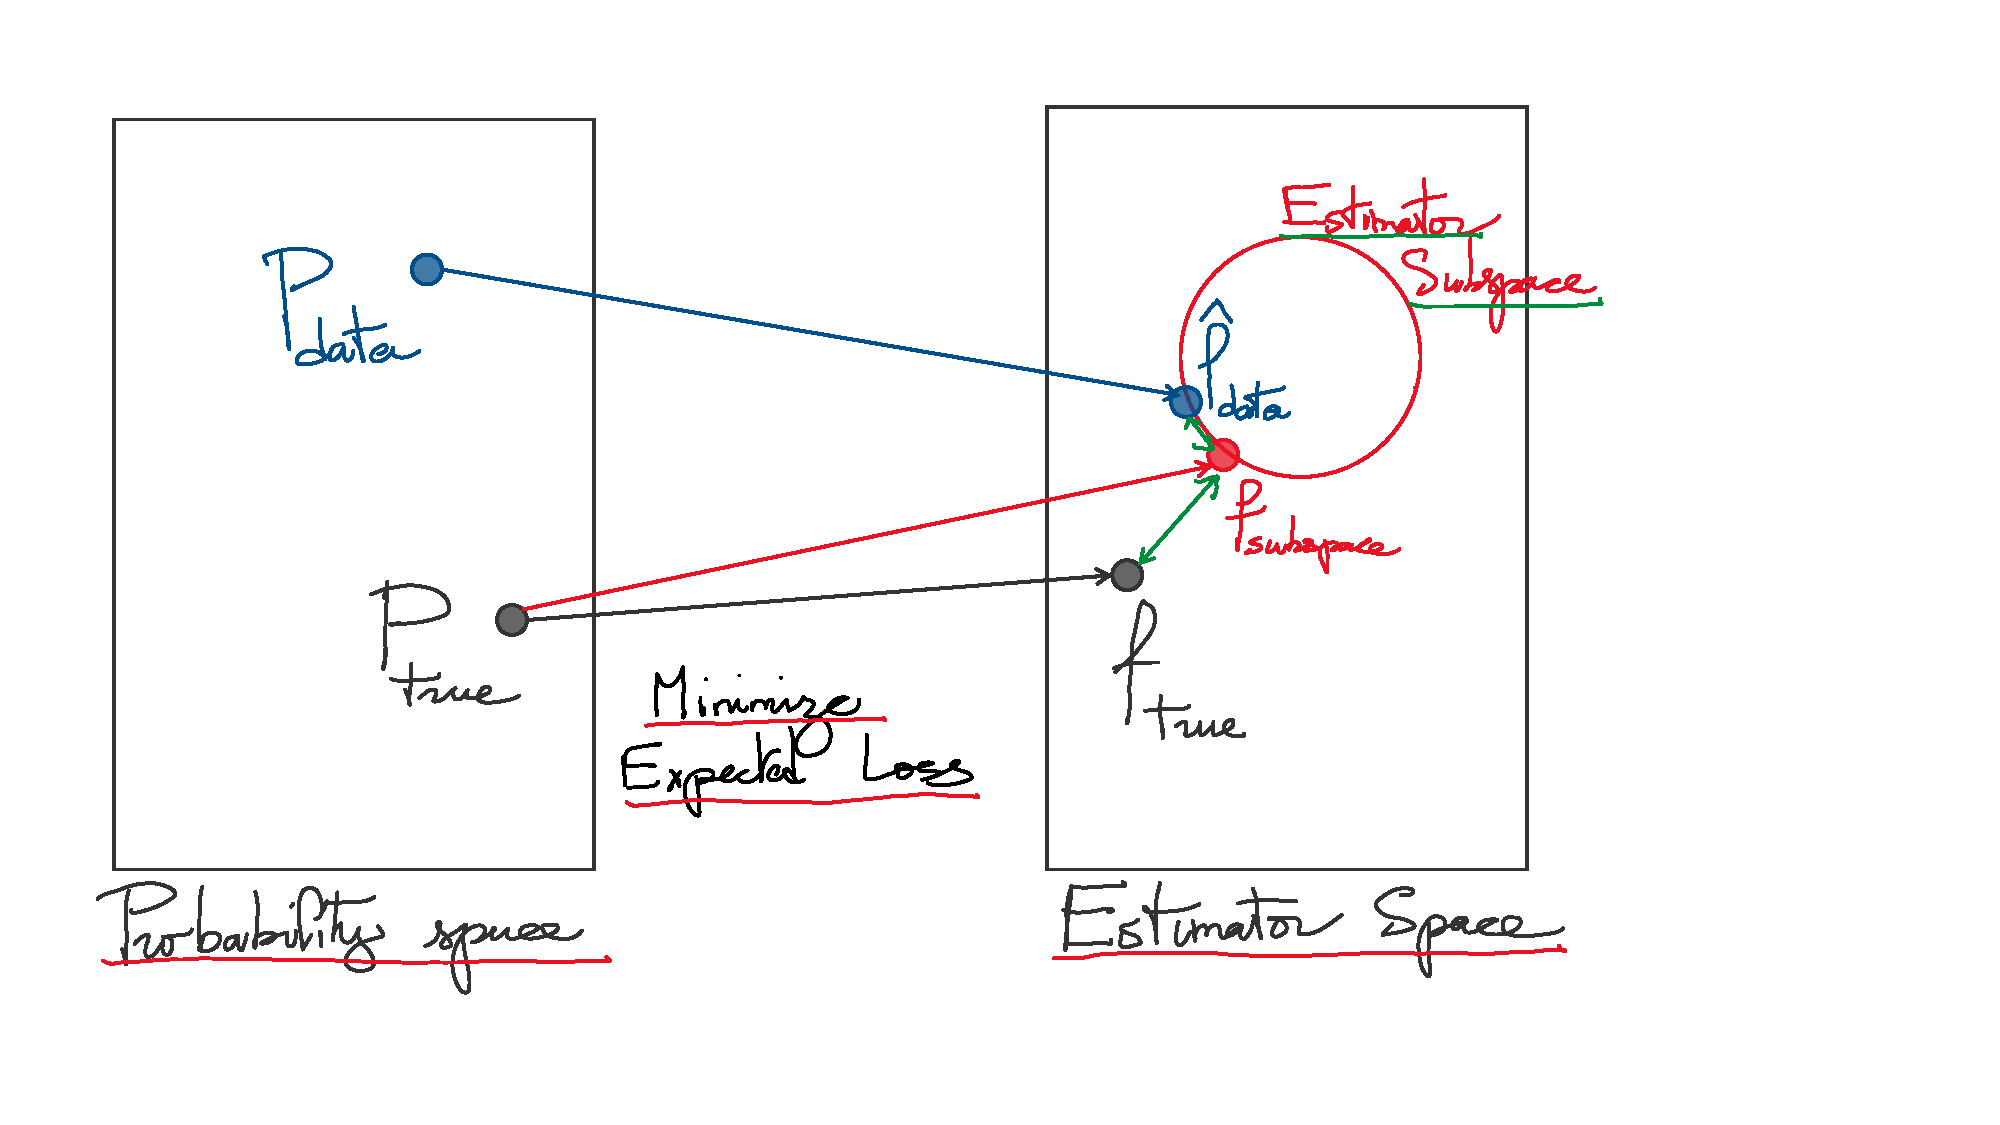
\includegraphics[trim=1cm 1cm 5cm 1cm,clip,width=\textwidth]{Figures/learning_fig.pdf}
\caption{\label{fig:bias_var} Sources of errors in statistical Learning: When $P^*$ is the distribution of the data, the optimal predictor $f^*$ minimizes the expected loss function. Based on data $Z_1, \ldots, Z_N$, the sample-based distribution is $\hat P = (\de_{Z_1} + \cdots + \de_{Z_N})/N$ and the empirical loss is minimized over a subset $\CS$ of the space of all possible estimators. The expected discrepancy between the resulting estimator and the  one minimizing the true expected loss on the subspace  is the ``variance'' of the method, and the expected discrepancy between this subspace-constrained estimator and  and the optimal one is the ``bias.''
}
\end{figure}

\begin{remark}
\label{rem:bias}
If the assumption made on $\hf^*$ is not valid, one can  write
\[
R(\hf_N)= \myE(|Y- \hf_N(X)|^2) \leq  2\big(\myE(|Y- \hf^*(X)|^2) + \myE(|\hf_N(X) - \hf^*(X)|^2)\big) 
\]
and still obtain a control (as an inequality) of the generalization error by a bias-plus-variance sum.
\end{remark} 

%\section{Classification}
%
%The context of classification is exactly the same as that of regression,
%except that the predicted variable, $Y$, is categorical,  taking values in a finite set, $\CR_Y$, of
%classes. The classifier is therefore a function $f:\CR\to \CR_Y$.
%The difference with the previous case is that loss functions used
%with quantitative variables are not adapted to classification (if
%the class labels represent vehicles, for example, the
%expression $(\text{car} - \text{truck})^2$ is
%meaningless). The most commonly used function in this context is the
%0\,--\,1 loss
%$$
%r(y,y') = 1 \text{ if } y\neq y', \text{ and 0 otherwise}.
%$$
%
%Using this loss function yields the average risk
%$R(f)   = 1 - P(Y=f(X))$ so that optimal functions $f$  have to maximize the rate
%of good classification: $P(Y=f(X))$. Similar to the case of regression,
%we can write
%$P(Y=f(X)) = E(P(Y=f(X) |X))$ and the optimal estimator must satisfy
%$$
%f_*(x) = \mathrm{argmax}\{P(Y=c|X=x): c\in \CR_Y\}
%$$
%This provides the maximum {\em a posteriori} (MAP) estimator given by the
%mode of the posterior distribution, which is the conditional
%distribution of the output given the observation. It is also called
%the Bayes estimator. But it only has a theoretical use, since the
%conditional distribution of $Y$ given $X$ is unknown. Similar to
%regression, generative and discriminative approaches exists, as well
%as a bias-variance trade-off. Many related issues will be discussed in the remaining
%of this course.

\section{Evaluating the  error}
\label{sec:error}

\subsection{Generalization error}
Given input and output variables $X:\Om\to \CR_X$ and $Y:\Om\to\CR_Y$ and a risk function $r: \CR_Y\times \CR_Y \to [0. +\infty)$, we have defined the generalization (or prediction) error as
$$
R(f) = \myE(r(Y, f(X)))\,.
$$
Recall that a training set $T = ((x_1, y_1), \ldots, (x_N, y_N))$ is a realization $T = \mT(\om)$ of  the random variable $\mT=((X_1, Y_1), \ldots, (X_N,
Y_N))$, an i.i.d. sample of the joint distribution of $(X,Y)$. A {\em learning algorithm} is a function $T \mapsto \hf_{T}$ defined on the set of training sets, namely, $\bigcup_{N=1}^\infty (\CR\times\CR_Y)^{N}$ and taking values in $\CF$.  


For a given $T$ and a specific algorithm, one is primarily interested in evaluating $R(\hf_{T})$, the generalization error of the predictor estimated from observed data.  To emphasize the fact that the training set is fixed in this expression, one often writes:
\[
R(\hf_{T}) = \myE(r(Y, \hf_{\,\mT}(X)) | \mT = T)
\]

If we  also take the expectation with respect to $T$ (for fixed $N$), we obtain the averaged generalization risk as
\[
\myE(R(\hf_{\,\mT})) = \myE(r(Y, \hf_{\,\mT}(X))),
\]
which provides an evaluation of the average quality of the algorithm when evaluated on random training sets of size $N$.
If $A: T \mapsto \hf_{T}$ denotes the learning algorithm, we will denote $\overline R_{N}(A) = \myE(R(\hf_{\,\mT}))$.

Since their computation requires the knowledge of the joint distribution of $X$ and $Y$, these errors are not available in practice. Given a training set $T$ and a predictor $f$, one can compute the empirical error
\[
\hat R_T(f) = \frac{1}{N} \sum_{k=1}^N r(y_k, f(x_k))\,.
\]
Under the usual moment conditions, the law of large numbers implies that $\hat R_{\,\mT}(f) \to R(f)$ with probability one for any given predictor $f$.  However, the law of large numbers cannot be applied to assess whether the {\em in-sample error},
\[
\CE_T \defeq \hat R_T(\hf_T) = \frac{1}{N} \sum_{k=1}^N r(y_k, \hf_T(x_k)),
\]
is a good approximation of the generalization error $R(\hf_T)$. This is because each term in the sum depends on the full data set, so that $\CE_\mT$ is not a sum of independent terms. The in-sample error typically under-estimates the generalization error, sometimes with a large discrepancy.

When one has enough data, however, it is possible to set some of it aside to form a test set.
Formally, a test set is a collection $T' = (x'_1, y'_1, \ldots, x'_{N'}, y'_{N'})$ considered as a realization  of an i.i.d. sample of $(X,Y)$, $\mT' = (X'_1, Y'_1, \ldots, X'_{N'}, Y'_{N'})$, independent of $\mT$.
 The test set error is then given by
\[
\CE_{T, T'}  = \hat  R_{T'}(\hf_T) = \frac{1}{N'} \sum_{k=1}^{N'} r(y'_k, \hf_T(x'_k)).
\]
The law of large numbers (applied conditionally to $\mT = T$) implies that $\CE_{T,\mT'}$ converges to $R(\hf_{T})$ with probability one when $N'\to \infty$.

However, in many applications, data acquisition is difficult or expensive (e.g., in the medical field) and sparing a part of it in order to form a test set is not a reasonable option. In such situations, cross-validation is generally a preferred alternative.


%\subsection{In-sample error}
%\label{sec:is.err}
%Both variables $X$ and $Y$ are assumed to be random in this setting,
%but there are often situations when one of them is ``more random'' than the
%other. Randomness on $Y$ is associated to measurement errors, or
%ambiguity in the decision.  Randomness in $X$ more generally relates to
%the issue of sampling a dataset in a large dimensional space. In some
%cases, $Y$ is not random at all: for example, in object recognition,
%the question ``is this a pipe?'' in Fig. \ref{fig:pipe} has a deterministic answer. 
%
%Sometimes, $X$ is small dimensional and densely sampled, but $Y$ is subject to noise. In such cases (which
%are unfortunately not the most interesting ones in modern machine
%learning), one can define the in-sample generalization error given by
%$$
%\CE'(T) =  \frac{1}{N} \sum_{k=1}^N E(r(Y', \hf_T(x_k)) | T, X = x_k).
%$$
%In this expectation, $T$ (and therefore $\hf_T$) is fixed, and the
%expectation is over $Y'$, which follows the conditional distribution
%of $Y$ given $X=x_k$. This corresponds  to averaging over
%new training sets, when one keeps the same input variables, but generates
%new outputs.
%
%\begin{figure}
%
\includegraphics[width=0.6\textwidth]{Figures/MagrittePipe.jpg}
%\caption{\label{fig:pipe} The treachery of images, by Magritte. The text says "this is not a pipe". (Reproduced without permission.)}
%\end{figure}
%
% 
%Consider the case of a square error $r(y, y') = (y-y')^2$. We have
%\begin{eqnarray*}
%\CE'(T) &=&   \frac{1}{N} \sum_{k=1}^N E((Y'_k - \hf_T(X_k))^2 | T)\\
%&=& \frac{1}{N} \sum_{k=1}^N E((Y'_k - Y_k + Y_k - \hf_T(X_k))^2 | T)\\
%&=& \CE(T)  - \frac{2}{N} \sum_{k=1}^N E((Y'_k - Y_k) \hf_T(X_k) | T)+  \frac{1}{N} \sum_{k=1}^N E ( (Y'_k)^2 - Y_k^2 | T)\\
%\end{eqnarray*}
%Write $T = (\CX, \CY)$ to separate the predictor and predicted variables in the training set. We compute the ``expected optimism,'' given by
%\[
%E(\CE'(T) - \CE(T)|\CX) =  - \frac{2}{N} \sum_{k=1}^N E((Y'_k - Y_k) \hf_T(X_k) | \CX)+  \frac{1}{N} \sum_{k=1}^N E ( (Y'_k)^2 - Y_k^2 | \CX)
%\]
%(so that expectation is taken for the conditional distribution of $\CY$ given $\CX$).
%The last term vanishes because $Y$ and $Y'$ have the same distribution given $\CX$. We have
%\begin{align*}
%E((Y'_k - Y_k) \hf_T(X_k) | \CX) &= E(Y'_k|\CX)E(\hf_T(X_k(|X) - E(Y_k \hf_T(X_k) | \CX)\\
% &= -\mathrm{cov}(Y_k, \hat f_T(X_k)|\CX)
%\end{align*}
%in which we have used the fact that $Y'_k$ and $\CY$ are conditional independent given $\CX$ and that $Y_k'$ and $Y_k$ have the same distribution, still conditional to $\CX$. We therefore find
%\[
%E(\CE'(T) - \CE(T)|\CX) = \frac{2}{N}\mathrm{cov}(Y_k, \hat f_T(X_k)|\CX).
%\]
%We will see in Chapter
%\ref{chap:ms} how the expected optimism can be used to penalize the training
%error and often improve the reliability of the estimators.


\subsection{Cross validation}

\subsubsection{Cross-validation error}
The $n$-fold cross-validation method (see, e.g., \citet{stone1974cross}) separates the training set into $n$ non-overlapping
sets of equal sizes, and estimates $n$ predictors by leaving out one
of these subsets as a temporary test set. A generalization error is 
estimated from each test set and averaged over the $n$ results.  

Let us formalize this computation after introducing some notation. We represent training data in the form $T = (z_1, \ldots, z_N)$, a sample of a random variable $Z$. With this notation, we can include supervised problems, such as prediction (taking $Z = (X,Y)$) and unsupervised ones such as density estimation (taking $Z=X$). One tries to estimate a function $f$ within a given class (e.g., a predictor, or a density) and one has a measure  of ``loss'', denoted $\ell(f, z)\geq 0$ measuring how badly  $f$ performs on the data $z$. For prediction, one takes $\ell(f, z) = r(y, f(x))$ with $z = (x,y)$ and for density estimation, e.g., $\ell(f, z) = - \log f(z)$, the negative log-likelihood. One then lets $R(f) = E(\ell(f, Z))$.  For an algorithm $A: T\mapsto \hat f_T$, the loss $\bar R(A)$ is the quantity of interest. 


Given another set $T' = (z'_1, \ldots, z'_{N'})$, the empirical loss is 
\[
\hat R_{T'}(f) = \frac1{N'} \sum_{k=1}^{N'} \ell(f, z_k')
\]
and, using $T$ as a training set and $T'$ as a test set, we let
\[
\CE_{T,T'} = \hat R_{T'}(\hf_T).
\]

To define an $n$-fold cross-validation estimator of the error, one assumes that the training set $T$ is partitioned into $n$ subsets of equal sizes (up to one element if $N$ is not a multiple of $n$), $T_1$, \ldots, $T_n$, so that $T_i$ and $T_j$ are non-intersecting if $i\neq j$, and $T = \bigcup_{i=1}^n T_i$.  For each $i$, let $T^{(i)} = T\setminus T_i$, which provides the training data with the elements of $T_i$ removed. Then, the $n$-fold cross-validation error is defined by
\[
\CE_{\mathrm{CV}}(T) = \frac1n \sum_{i=1}^{n} \CE_{T^{(i)}, T_i}\,.
\]

Assuming, to simplify, that $N$ is a multiple of $n$, the expectation of the cross-validation error is $E( R (\hat f_{\mT_{N'}}))$, where the average is made over training sets $\mT_{N'}$ of size $N' = N-N/n$. Note that the cross-validation error is an estimate of the average error of the algorithm over random training sets, not necessarily that of the current estimator $\hf_T$. It returns an evaluation of the algorithm $A: T\mapsto \hf_T$. When needed, one can emphasize this and write $\bar R_{\mathrm{CV}, T}(A)$.

The limit case when $n=N$ is called
leave-one-out (LOO) cross validation. In this case $\CE_{\mathrm{CV}} $ is an almost unbiased estimator of $E( R (\hf_{\boldsymbol T}))$, but, 
because it is an average of functions of the training set that are quite similar (and that will therefore be positively correlated), its variance (as a function of $T$) may be quite large. Conversely, smaller values of $n$ will have smaller variances, but larger biases. In practice, it is difficult to assess which choice of $n$ is optimal, although 5- or 10-fold cross-validation is quite popular. LOO cross-validation is also often used, especially when $N$ is small.

\subsubsection{Model selection using cross validation}

Because it evaluates the quality of an algorithm, cross-validation is often used to perform model selection. Indeed, many learning algorithms depends on a parameter, that we will denote $\la$. In kernel density estimation,  for example, $\la=\sig$ is the kernel width. For mixtures of Gaussian, $\la =m$ is the number of Gaussian terms in the mixtures. Formally, this means that one has, for every $\la$, an algorithm $A_\la: T \mapsto \hf_{T, \la}$. 


Fixing a training set $T$, one can compute, for each $\la$,  the  cross-validation error $e_T(\la) = \bar R_{\mathrm{CV}, T}(A_\la)$. Model selection is then performed by finding 
\[
\la^*(T) = \argmin_\la e_T(\la). 
\]
Once this $\la^*$ is obtained, the final estimator is $\hf_{T, \la^*(T)}$, obtained by rerunning the algorithm one more time on the full training set. 

This defines a new training algorithm, $A^*: T \mapsto \hf_{T, \la^*(T)}$. It is a common mistake to consider that the cross-validation error associated to this algorithm is still given by $e(\la^*(T))$. This is false, because the computation of $\la^*$ uses the full training set. To compute the cross-validation error of $A^*$, one needs to encapsulate this model selection procedure in an other cross-validation loop. So, one needs to compute, using the previous notation,
\[
\CE^*_{\mathrm{CV}}(T) = \frac1n \sum_{i=1}^n \hat R_{T_i}(\hf_{T^{(i)}, \la^*(T^{(i)})})
\]
where each $\hf_{T^{(i)}, \la^*(T^{(i)})}$ is computed by running a cross-validated model selection procedure restricted to $T^{(i)}$. This is often called a double-loop cross-validation procedure (the number of folds in the inner and outer loops do not have to coincide). 
Note that each $\la^*(T^{(i)})$ that does not necessarily coincide with the optimal $\la^*(T)$ obtained with the full training set. 


